\chapter{First Design Guidelines Development}\label{C:bin}

In section 2.2, we presented Transactional Distance Theory (TDT), the elements: dialogue, course structure, and learner autonomy that varied transactional distance and how these affected learning quality. However, TDT was proposed within distance education context. This chapter therefore firstly presents analysis of applicability of TDT to m-learning context. Additionally, in section 2.3, we presented other learning theories that had potential to complement TDT and improved design guidelines of m-learning. This chapter therefore secondly presents applicability of the other learning theories to m-learning guidelines. Ultimately, as stated in section 2.4 that TDT lacked of usability guidelines regarding interface design. This chapter therefore presents usability design design of m-learning. The next section of this chapter presents the first design guidelines developed from the combination of TDT, complementation of other learning theories, and usability design regarding interface design. Following the guidelines, in the last section, we presents a mobile learning application design. 
\newpage 
\section{Applicability of TDT to M-learning} 

Transactional Distance Theory (TDT) was proposed in distance education which was an umbrella term that encompassed mobile learning (m-learning). However, m-learning had some unique characteristics of mobility and limitations of mobile devices, adopting TDT within m-learning context might require some clarifications regarding TDT's applicability to m-learning. This section presents analysis of applicability of TDT to m-learning starting by analysis of related terms, analysis of relationships between the elements and transactional distance, and analysis of potentials of mobile devices to accommodate six instructional process of m-learning. 


Firstly, Table 4.1 presents of TDT-related terms originally defined by Moore (1993) \cite{moore1993theory} and analysis of its applicability to m-learning context. 
\newpage 
\begin{table}[H]
\centering
\caption{applicability of TDT to m-learning}
\begin{tabular}{ |p{2.3cm}|p{4 cm}|p{6.2 cm}|} 
 \hline
Term & Original Concept \cite{moore1993theory} & M-learning Context  \\ 
\hline
Transactional Distance & Learners perceived isolation due to some hardship to communicate with their teachers & The isolation were likely to be lessen as mobile devices were capable to provide both synchronous (e.g., voice and video calling) and asynchronous communication (e.g., email) and not only with teachers but also with others learners  \\ 
\hline
 Dialogue & Interaction including words and actions that had positive quality purposeful, and constructive  & Even though mobile devices could cater quicker, easier communication, and multiple interaction of words and action simultaneously, the extent of the dialogue should yet had positive quality purposeful, and constructive \\ 
 \hline
 Course Structure & Structural plan of the course the informed how learning content would be delivered through communication media & M-learning adopted mobile devices to deliver learning content, therefore possible media were text, recorded audio, and video presentation \\ 
\hline
 Learner Autonomy & Learners' ability to determine learning goals and make decision on learning process & Besides these abilities, m-learning involved mobile devices therefore abilities and willingness to use the devices to learn should also included into the autonomy \\ 
 \hline
\end{tabular}
\end{table}
\newpage 
Secondly, besides introducing transactional distance and its related elements, Moore (1993) \cite{moore1993theory} also proposed relationships between these elements and explained how it affected learning quality. The following list summarizes the Moore (1993) \cite{moore1993theory}'s proposition and presents how its capability to m-learning. 

\begin{enumerate} 
\item \textbf{The course that had high degree of structure (inflexible) and allowed little to no dialogue had high transactional distance}
\newline M-learning had capability to allow teachers to control all learning processes from setting learning goal, implementing learning, and evaluating learning outcomes. In the implementing process, teachers could, for example, allow learners to explore only some part of learning content and lock the access to the rest of the content or allow learners to access to the content in pre-arrange schedule. These was an inflexible course that allowed the teachers to control learners' learning pace and schedule. Additionally, if this inflexible m-learning course did allow the learners to have a successful dialogue with their teachers. Learners, for example, sent an e-mail to a teachers or submitted an electrical assignment but did not received any reply or feedback from the teachers, they might perceived transactional distance and these might decrease m-learning quality. 

\item \textbf{The course that has flexible structure and allowed dialogue had less transactional distance} 
\newline M-learning had capability to allow learners to control all learning process from setting learning goals, implementing learning, and evaluating learning outcomes while teachers could be facilitators that support the learning process. In the implementation process, for example, learners could access to all learning materials whenever they wanted to. These was a flexible course that allowed the learners to learn on their own pace and manage thir own learning schedule. Additionally, if this flexible m-learning course allowed the learners to have some positive quality, purposeful, and constructive dialogue with their teachers. Learners, for example, sent an e-mail and receive a reply from their teachers that helped them get a better understanding of the learning topic, they would not perceive transactional distance and these might increase m-learning quality. 

\item \textbf{Autonomous learners seems to be comfortable with less dialogue and less structural programme, meanwhile, non-autonomous learners seems to prefer more dialogue and more structural programme}
\newline As listed in number 1. and 2., m-learning had potential to provide dialogue and either firm or flexible structure to learners. Therefore, observing learner autonomy at the early stage of the design process is necessary for designing suitable m-learning to learners

\end{enumerate} 


Ultimately, Moore (1993) \cite{moore1993theory} suggested six instructional process that should be included into a distance education course (Section 2.2.3). M-learning design on mobile devices had capability to present these instructional processes. Table 4.2 presents the capability of mobile devices to accommodate the six instructional processes. 
\newpage 
\begin{table}[!htb]
\centering
\caption{Mobile devices' capability to accommodate instructional process of m-learning}
\begin{tabular}{ |p{2.6 cm}|p{9.9 cm}|} 
 \hline
Instructional Process \cite{moore1993theory} & Capability \\ 
\hline
Presentation & Mobile devices could present electrical media such as text on screen, recorded audio  \\ 
\hline
Motivation & Mobile device had many communication features such as texting service, e-mailing, voice and video calling that teachers could used to send learners some feedback, motivate and encourage learners to learn \\ 
 \hline
Stimulation of Analysis and Criticism & Teachers could arrange an on-line discussion with a group of learners, send them a pre-recording of experts' discussion and learners could easily access to video-sharing website such as YouTube to watch some academic debates \\ 
\hline
Advice and Consolation & Same with the motivation process, teachers could use all these communication features to advice and provide personal consultation to learners   \\ 
 \hline
Practice and Evaluation & Learners could practice what they have learnt by having some discussion with their teachers though the communication features, challenging themselves with game-based learning, or performing some assignments. Teachers' feedback could be used as a self evaluation for the learners \\ 
 \hline
Creation of Knowledge &  Same with the motivation process, learners could use the communication features to discuss and share their ideas with their teachers \\ 
 \hline
\end{tabular}
\end{table}


\section{Applicability of Other Theories to M-learning} 

Even though, TDT had capabilities to guide m-learning design and mobile devices also had capabilities to accommodate m-learning dialogue and instructional process of m-learning.There were some other learning theories discussed in Section 2.3 that would complement TDT and contribute to a better design decision. The following list presents contributions of other learning theories to m-learning design. 

\begin{enumerate} 
\item Cognitive Load Theory - suggesting how to present learning tasks to reduce working memory load \cite{sweller1998cognitive}
\begin{itemize}
\item If learners had low level of prior knowledge about the learning topic, present learning tasks with progressive method (presenting easy task first and add more complexity to the task later) \cite{clarke2005impact}
\item Take caution on presenting animation in m-learning. If learners had low prior knowledge about the learning topic, presenting learning content with animation might decrease germane cognitive load which was important cognitive process for learning \cite{schnotz2005enabling}
\end{itemize} 
\item Self-Determining Theory - providing a better understanding of learners' cognitive that help teachers appropriately motivate learners \cite{ryan2000intrinsic}
\begin{itemize} 
\item Learners' intrinsic motivation could be triggered by providing challenge, curiosity, control, fantasy, cooperation, competition, and recognition within learning tasks \cite{malone1987making}
\item Learners' extrinsic motivation could be triggered by some external rewarding such as good grades and scholarships \cite{ryan2000intrinsic}
\item If learners had already found that the learning was intrinsically rewarding, the extrinsically rewarding should not be applied \cite{rosenfield1980rewards} 
\end{itemize} 
\item Media Richness Theory - raising awareness toward presenting multi media because, even though, it could facilitate share understanding and clarify ambiguity of communication, too much of them are distracting \cite{daft1983information} and \cite{sun2007design}. 
\begin{itemize} 
\item For high ambiguous and uncertain learning content, the rich media such as animation would be appropriate. Meanwhile, for the low ambiguous and uncertain learning content, the rich media was not necessary \cite{sun2007design}
\end{itemize}
\item Learning Theory of Andragogy - raising awarenesses that maturity had significant effects on how learners learnt \cite{knowles1970modern} and adult learners have have their own cognitive process and would be motivated differently to children learners \cite{cercone2008characteristics}. 
\item Activity Theory and Culturak-History Activity Theory - providing understanding that human learners were enculturated, therefore m-learning design should consider their history path of behavior and the learners' development processed were interlinked in both individual and social levels. The socio-cultural learners would approach m-learning using mobile devices as instruments with some facilitations provided by teachers. 

\end{enumerate} 

\section{Usability Design of M-learning} 

In order to design for usability, we adopted the eight golden rules of interface design \cite{shneiderman2010designing}: 
\begin{itemize} 
\item Provide language and interaction consistency 
\item Enable users to use shortcut 
\item Offer informative feedback
\item Design dialogue to inform users where they are, what they are doing, and provide closure dialogue when they accomplished any task 
\item Provide simple error handling mechanism 
\item Permit easy reversal of action if users make any input mistake 
\item Allow users to feel in control over the system
\item Reduce short-term memory load 
\end{itemize} 

Additionally, with regards to the small display and mobility mobile devices, we also included some interface design guidelines for mobile devices proposed by  Gong \& Tarasewich (2004) \cite{gong2004guidelines} and Jones \& Marsden (2006) \cite{jones2006mobile}: 

\begin{itemize} 
\item Design for dynamic context of use - provide alternative interactions and provide interface design that require as little attention as possible
\item Design for small devices - present learning content in hierarchical order 
\item Design for enjoyment - interface design should be useful, fun, and visual pleasing 
\end{itemize} 

\section{First M-learning Design Guidelines} 
Our m-learning design guidelines were mainly grounded on Transactional Distance Theory principles. It was complimented with some suggestion of other learning theories and the eight golden rules of interface design. Table 4.3 presents our first version of m-learning design guidelines. 

\begin{table}[H]
\centering
\begin{tabular}{ |p{13 cm}|} 
\hline
\textbf{1. Observe learner autonomy or perform learner study}\\
\hline 
As autonomous and non-autonomous learners prefer different course structure and require different quality and quantity of dialogue and maturity had significant effects on how learners learnt developers should have basic knowledge about learners to design an applicable application to them

\\
\hline
\end{tabular}
\end{table}


\begin{table}[!htb]
\centering
\begin{tabular}{ |p{13 cm}|} 
 \hline
 \textbf{2. Provide dialogue opportunities} \\ 
\hline
\begin{itemize}
\item Dialogue is used to provide feedback, advice and consultation to learners, motivate and encourage them to learn, and help them in their creation of knowledge \item Ensure that the dialogue were constructive, have positive quality, constructive, and allow learners to contributes to the dialogue 
\end{itemize}\\
\hline
\end{tabular}
\end{table}

\newpage

\begin{table}[!htb]
\centering
\begin{tabular}{ |p{13 cm}|} 
\hline 
\textbf{3. Provide flexible structure that suit learner autonomy}\\
\hline 
If learners are autonomous learners 
\begin{itemize} 
\item Teachers could initiate learning goals however ensure that learners were allowed to take part in goal setting process
\item Allow learners to learn at their own pace, manage their own learning schedule, and implement their own learning. 
\item Ensure that teachers role is a facilitator who provide feedback, consultations, advises, and other learning supports when learners require
\item Teachers could evaluate learners' knowledge to ensure learning quality however ensure that they are allowed to evaluate their own knowledge 
\end{itemize}
If learners are non-autonomous learners 
\begin{itemize} 
\item Teachers should set learning goals 
\item Teachers should allow a lot of dialogue opportunities, track learning progress, provide constructive encouragement and feedback, arrange advice and consultation schedule, and provide constructive learning material. 
\item Teachers should evaluate learners' knowledge to ensure learning quality
\end{itemize}\\
\hline 
\end{tabular}
\end{table}

\newpage 

\begin{table}[!htb]
\centering
\begin{tabular}{ |p{13 cm}|} 
\hline
\textbf{4. Choose appropriate media presentation}\\
\hline 
M-learning is capable to present multimedia
\begin{itemize} 
\item Ensure that the choice of media suit learners' capability 
\item Ensure that the choice of media suite learning content (i.e., high richness media such as animation only suits ambiguous learning learning content) and be caution that too much of media could be distracting 
\end{itemize} \\
\hline
\end{tabular}
\end{table}

\begin{table}[!htb]
\centering
\begin{tabular}{ |p{13 cm}|} 
\hline
\textbf{5. Motivate Learners}\\
\hline 
\begin{itemize} 
\item Provide learning tasks that are challenging and trigger learners' curiosity, competitiveness
\item If learners has no motivation toward learning topic and learning tasks adopt rewarding technique to increase their participation
\end{itemize} \\
\hline
\end{tabular}
\end{table}


\begin{table}[!htb]
\centering
\begin{tabular}{ |p{13 cm}|} 
\hline
\textbf{6. Allow learners to practice what they have learnt}\\
\hline 
\begin{itemize} 
\item Arrange some learning activities for learners to practice such as game-based learning or assignment
\item Ensure that they receive feedback on their performance 
\end{itemize} \\
\hline
\end{tabular}
\end{table}

\newpage 
\begin{table}[!htb]
\centering
\begin{tabular}{ |p{13 cm}|} 
\hline
\textbf{7. Design for usability}\\
\hline 
\begin{itemize} 
\item Provide language and interaction consistency 
\item Enable users to use shortcut 
\item Offer informative feedback
\item Design dialogue to inform users where they are, what they are doing, and provide closure dialogue when they accomplished any task 
\item Provide simple error handling mechanism 
\item Permit easy reversal of action if users make any input mistake 
\item Allow users to feel in control over the system
\item Reduce short-term memory load 
\item Design for dynamic context of use - provide alternative interactions and provide interface design that require as little attention as possible
\item Design for small devices - present learning content in hierarchical order 
\item Design for enjoyment - interface design should be useful, fun, and visual pleasing 
\end{itemize} \\
\hline
\end{tabular}
\end{table}


\newpage

\section{First Prototype Design}  

According to the first design guidelines, we designed the first m-learning application prototype

\subsection{Hardware and Software}
The application was design on iPhone 6s. figure 4.1 presents the iPhone size display specification. 

\begin{figure}[!hbt]\centering
    \begin{subfigure}{0.4\textwidth}
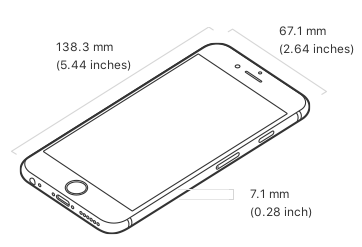
\includegraphics[width=\textwidth]{hw1}
\caption{Size}
    \end{subfigure}\hspace{0.05\textwidth}
 \begin{subfigure}{0.4\textwidth}
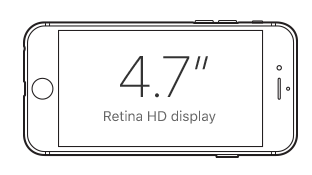
\includegraphics[width=\textwidth]{hw2}
\caption{Display}
 \end{subfigure}\hspace{0.05\textwidth}
  \caption{iPhone6s' s hardware specification \newline Figure taken from https://www.apple.com/nz/iphone-6s/specs/ on September, 2017}
\end{figure}

The iPhone 6s had iOS 10.2.1 and the first prototype was developed with an integrated developement environment Xcode 7.0.1 available on macOS

\subsubsection{1. Observe Learner Autonomy}
The actual autonomy of learners will be observed in laboratory setting (Chapter 5). At this stage of prototype development, we made an assumption about learner autonomy based on the primary persona (Clara) character. 

\begin{table}[H]
\centering
\caption{Learner autonomy and design plan}
\begin{tabular}{ |p{6.25 cm}|p{6.25 cm}|} 
 \hline
 Clara: ... & Design: ...\\ 
\hline
Had previous experiences using the text, recorded audio, and video as well as knew how to, for example play, pause, and fast forward, use the control function & Could accommodate text, recorded audio, and video presentation without any further advise from teachers, neither a manual guided how to used the media  \\ 
\hline
Appreciated that communication with her teachers would help improve her learning and she had already familiar with texting and emailing on the mobile devices & Could provide a chat function which would be used if learners had any questions without any further encouragement from teachers  \\ 
 \hline
Despite being appreciated that assignment had helped improve their learning, 
she preferred to do it on a desktop computer or laptop rather than a mobile phone & Adopt rewarding technique to extrinsically motivate learners to perform the assignment because they lacked of intrinsic motivation  \\ 
\hline
Had neutral attitude towards the game-based learning & Adopt rewarding technique to extrinsically motivate learners to play game-based learning because they lacked of intrinsic motivation  \\ 
 \hline
Seemed to be partially autonomous learners. Even though, she had no clear goal toward m-learning, they showed that they had ability to implement m-learning on their own & Provide dialogue opportunities and flexible course structure \\ 
 \hline
Unknown her autonomy towards evaluation process & Provide application features for self-evaluation (the game-based learning) as well as teachers evaluation (the assignment)  \\ 
 \hline
\end{tabular}
\end{table}

\newpage 
\subsubsection{2. Provide Dialogue Opportunities}
We design many-to-many chat function for learners. To maximize existing of dialogue and flexibility of course structure, learners were the one who initiate the chat. That is to say, they knew that the chat was available but it was their call if they would like to start conversion. Figure 4.2 presents design of chat function. The chat icon were available regularly therefore learners could use the chat wherever they were at their learning process. 

\begin{figure}[H]\centering
    \begin{subfigure}{0.27\textwidth}
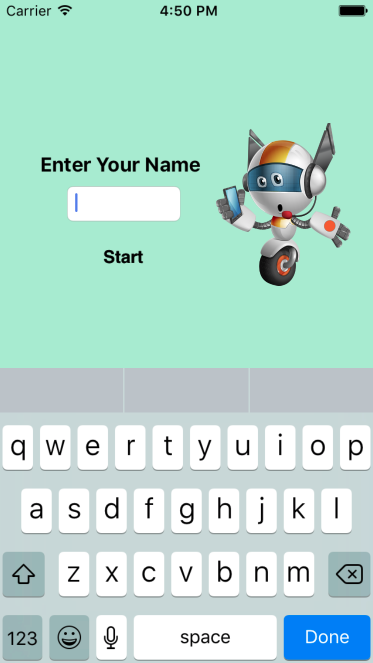
\includegraphics[width=\textwidth]{chat1}
\caption{Login Screen}
    \end{subfigure}\hspace{0.02\textwidth}
 \begin{subfigure}{0.27\textwidth}
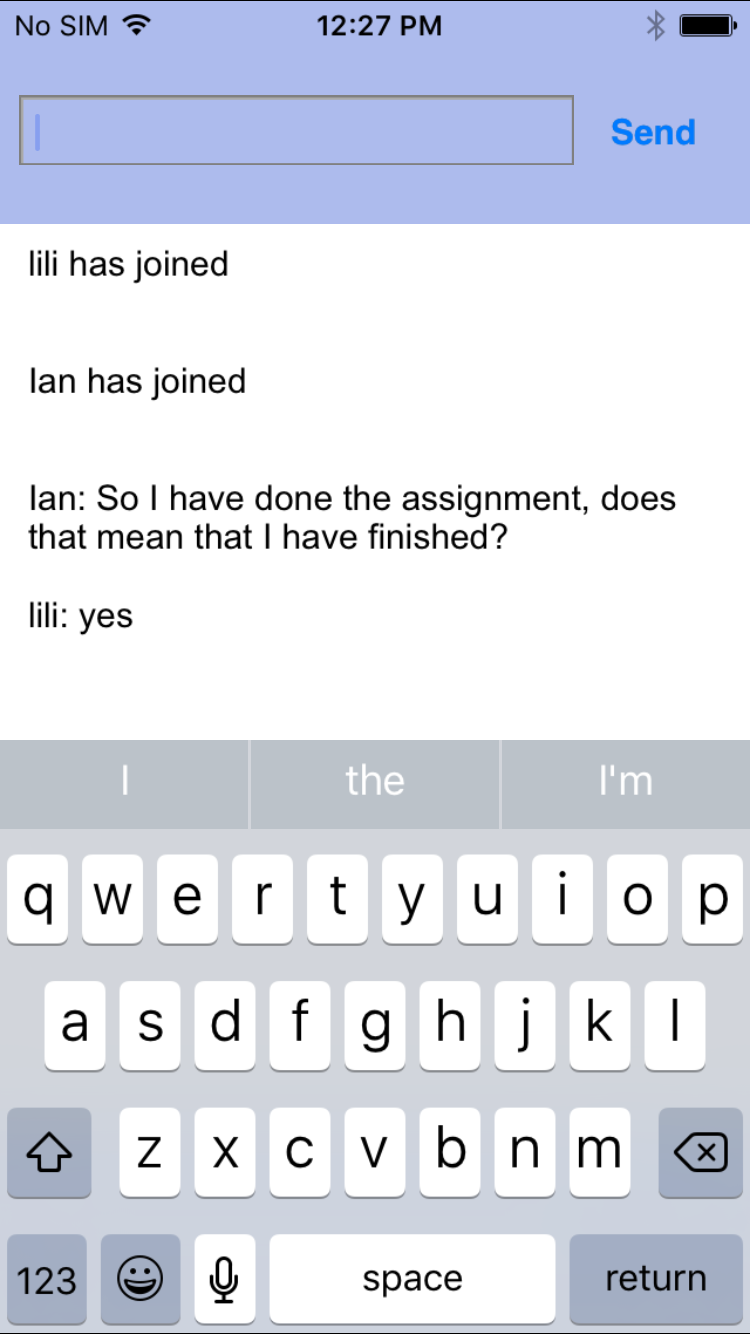
\includegraphics[width=\textwidth]{chat2}
\caption{Example of Chat}
 \end{subfigure}\hspace{0.5\textwidth}
 \begin{subfigure}{0.8\textwidth}
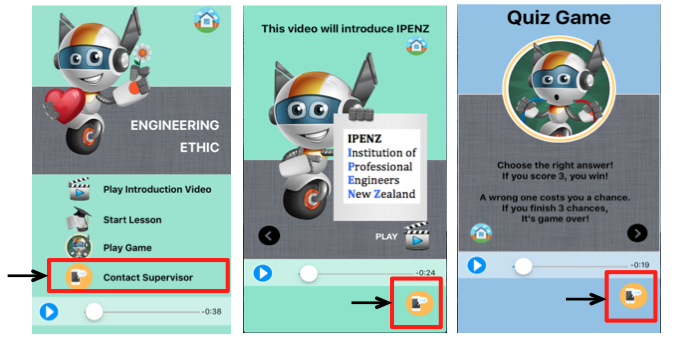
\includegraphics[width=\textwidth]{chat3}
\caption{Chat icon available along application design}
    \end{subfigure}\hspace{0.05\textwidth}
  \caption{Chat function design}
\end{figure}

\newpage 
\subsubsection{3. Provide flexible structure that suit learner autonomy}
As learners were assumed to be partially autonomous, therefore, teachers helped guiding the goal setting process by informing them at the beginning what they were about to learn, what activity they would perform and how it helped them to learn. However, as they showed that they had experience with with the media given within the application, they took control in the implementation process, with teachers acted as facilitator who provided assistance through chat if they required. In the evaluation process, we engage two mechanism, allow learners to evaluate themselves through the quiz game and we evaluate their understanding towards the learning topic using assignment. The assignment were analysis level that exercise their cognitive process. 

\begin{figure}[!hbt]\centering
    \begin{subfigure}{0.27\textwidth}
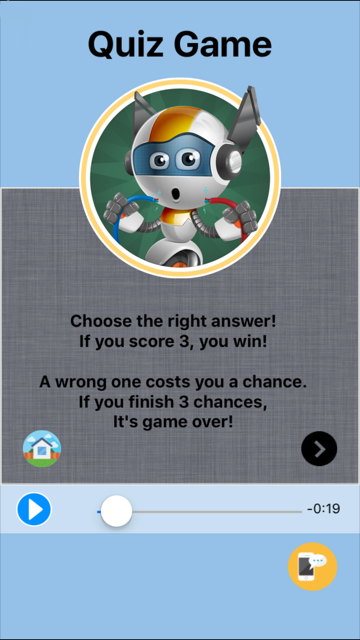
\includegraphics[width=\textwidth]{game1}
\caption{Introduction}
    \end{subfigure}\hspace{0.03\textwidth}
 \begin{subfigure}{0.27\textwidth}
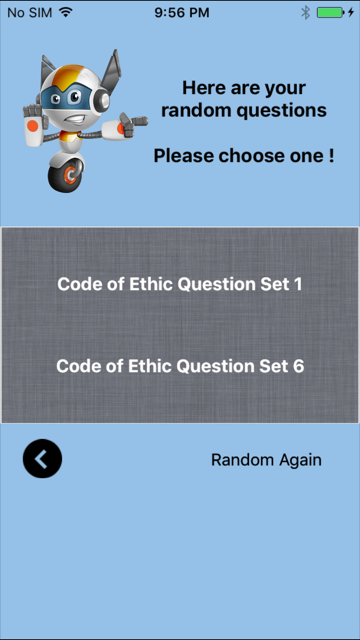
\includegraphics[width=\textwidth]{game2}
\caption{Categories}
 \end{subfigure}\hspace{0.03\textwidth}
 \begin{subfigure}{0.27\textwidth}
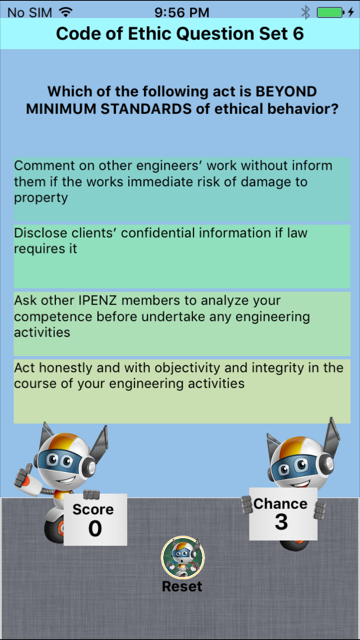
\includegraphics[width=\textwidth]{game3}
\caption{Multiple-choices}
    \end{subfigure}\hspace{0.05\textwidth}
  \caption{Game-based learning (Quiz Game) design}
\end{figure}
\newpage 
\begin{figure}[!hbt]\centering
    \begin{subfigure}{0.27\textwidth}
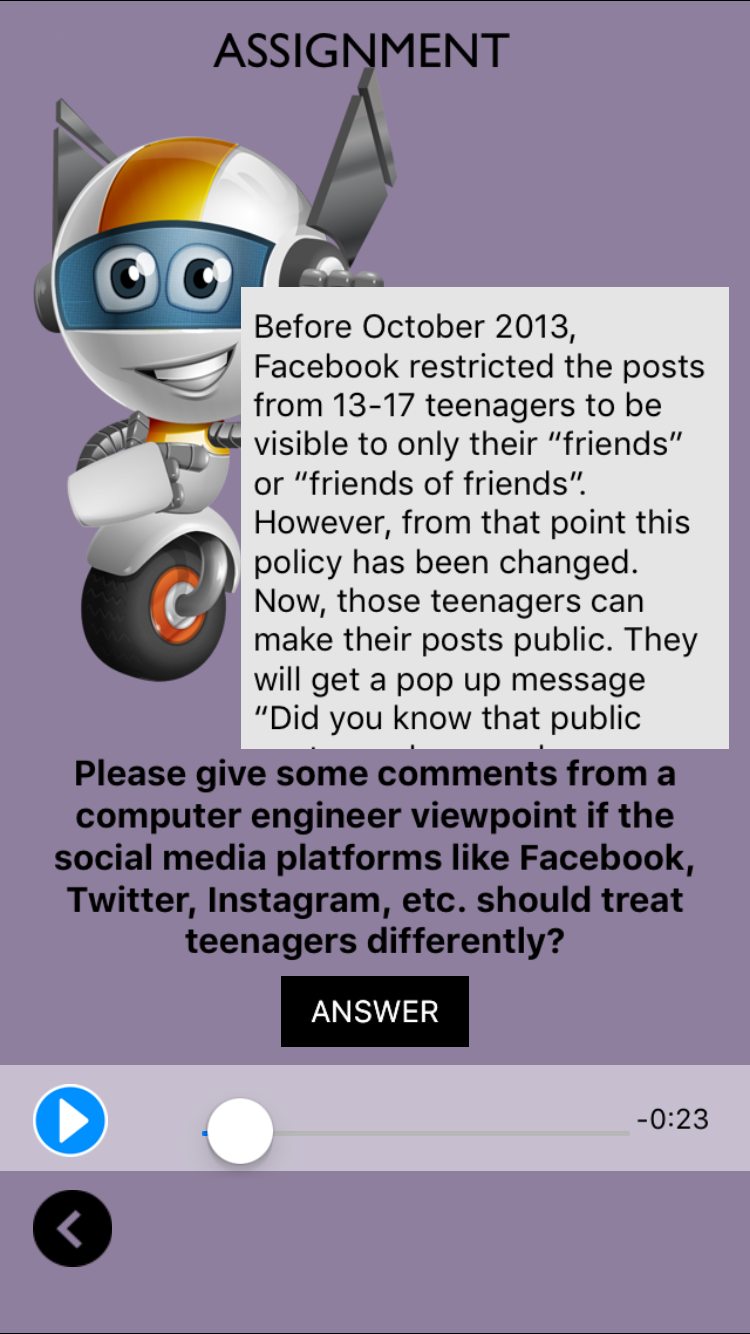
\includegraphics[width=\textwidth]{ass1}
\caption{Assignment}
    \end{subfigure}\hspace{0.06\textwidth}
 \begin{subfigure}{0.27\textwidth}
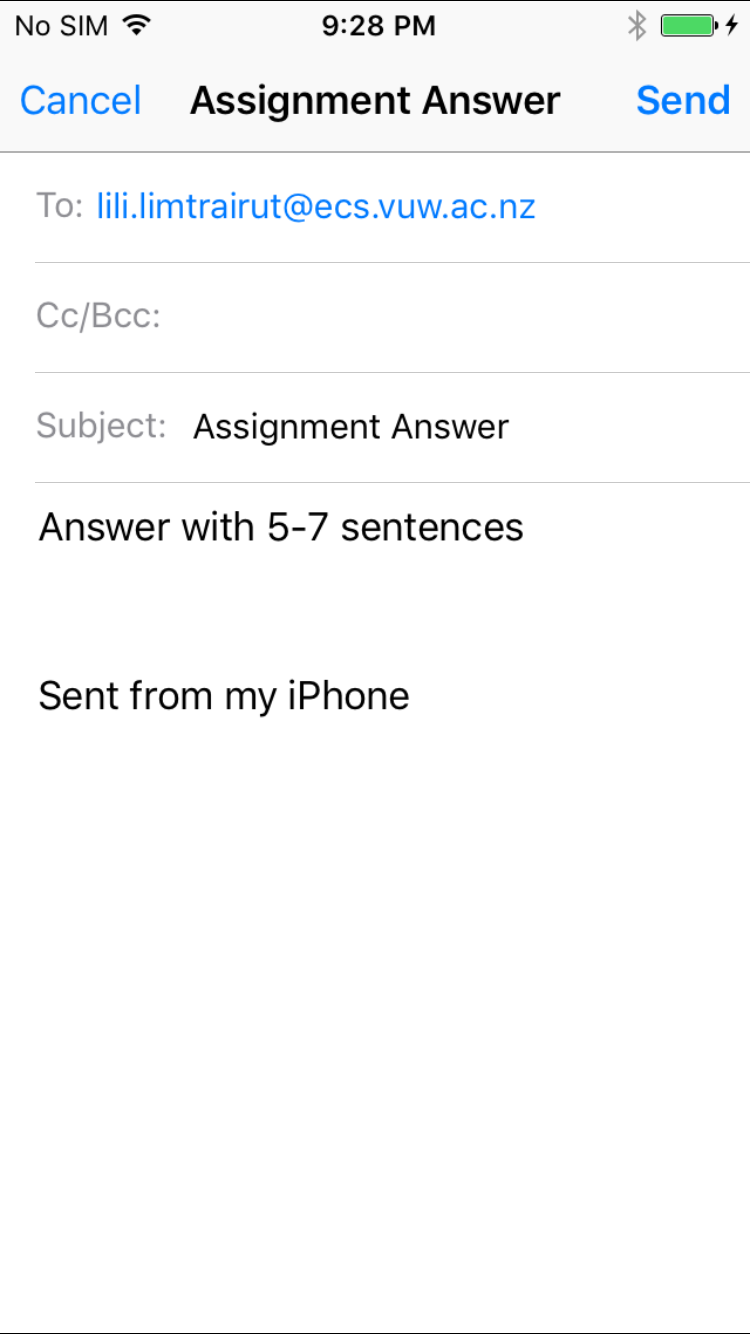
\includegraphics[width=\textwidth]{ass2}
\caption{Answer}
 \end{subfigure}\hspace{0.5\textwidth}
  \caption{Assignment (compulsary) design}
\end{figure}

\newpage 
\subsubsection{4. Choose appropriate media presentation}
We used text presentation to present learning content. Reading text were presented within textbox and learners could highlight and copy them. Recorded audio was used to introduce learning content and guided how to play the game-based function, perform the assigment, and the chat function. Animation video was used to introduce leaning content, encourage and motivate learners to learn. 

\begin{figure}[H]\centering
    \begin{subfigure}{0.27\textwidth}
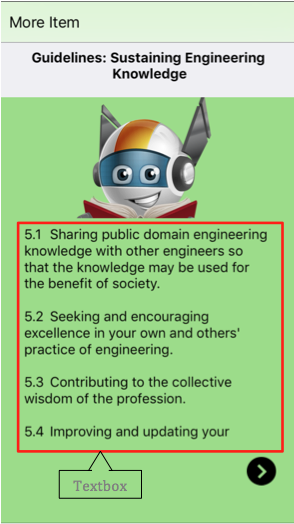
\includegraphics[width=\textwidth]{text1}
\caption{}
    \end{subfigure}\hspace{0.06\textwidth}
 \begin{subfigure}{0.27\textwidth}
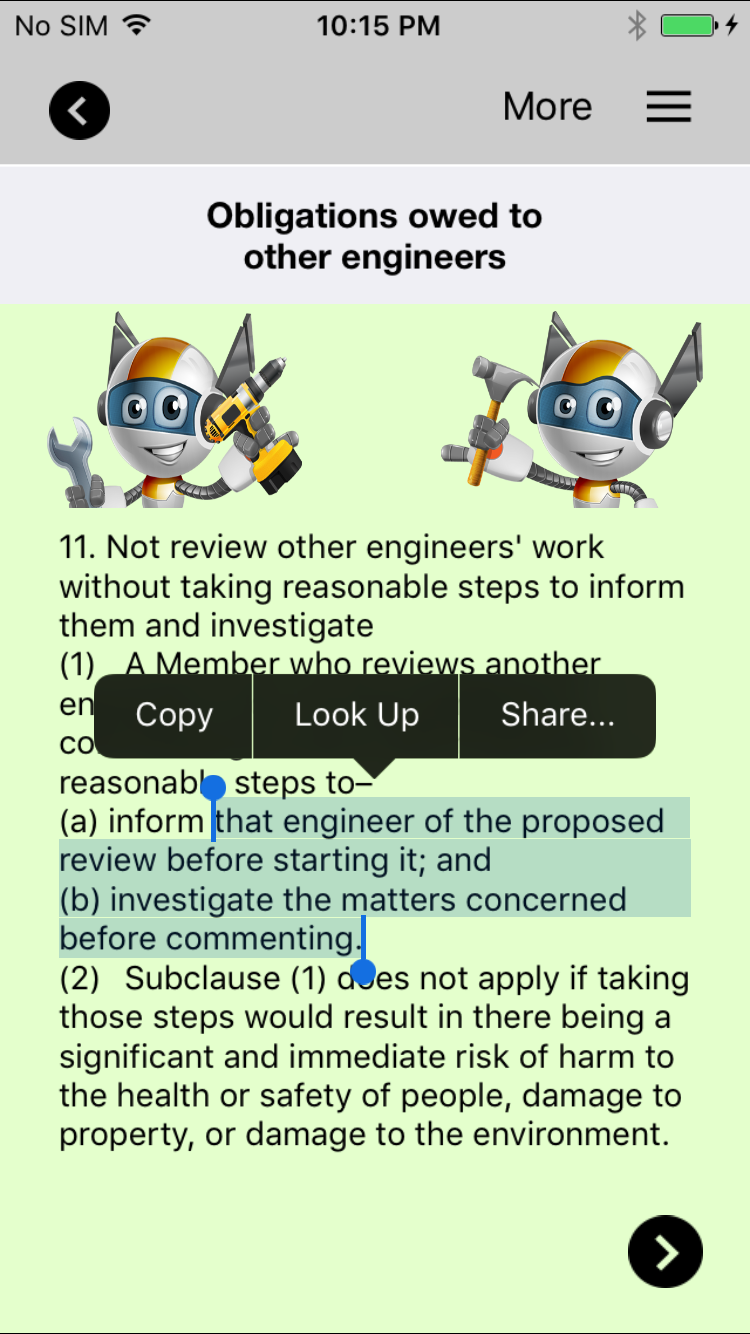
\includegraphics[width=\textwidth]{text2}
\caption{}
 \end{subfigure}\hspace{0.5\textwidth}
  \caption{Media text}
\end{figure}

\newpage 
\begin{figure}[H]\centering
    \begin{subfigure}{0.25\textwidth}
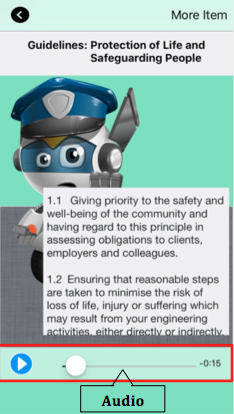
\includegraphics[width=\textwidth]{audio1}
\caption{}
    \end{subfigure}\hspace{0.03\textwidth}
 \begin{subfigure}{0.25\textwidth}
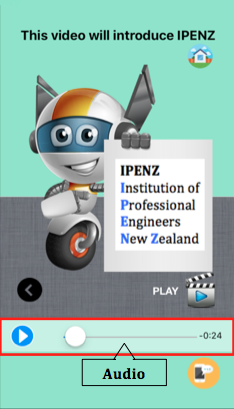
\includegraphics[width=\textwidth]{audio2}
\caption{}
 \end{subfigure}\hspace{0.03\textwidth}
 \begin{subfigure}{0.25\textwidth}
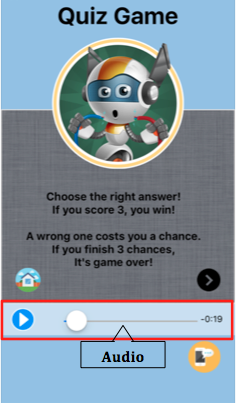
\includegraphics[width=\textwidth]{audio3}
\caption{}
    \end{subfigure}\hspace{0.03\textwidth}
  \caption{Examples of media recorded audio that introduces learning topic, available animation video, and quiz game}
\end{figure}

\begin{figure}[H]\centering
    \begin{subfigure}{0.25\textwidth}
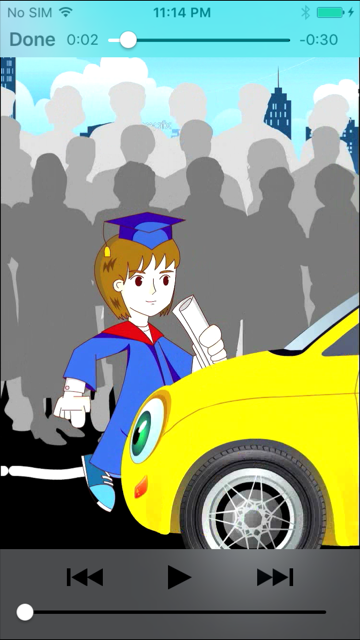
\includegraphics[width=\textwidth]{video1}
\caption{}
    \end{subfigure}\hspace{0.03\textwidth}
 \begin{subfigure}{0.25\textwidth}
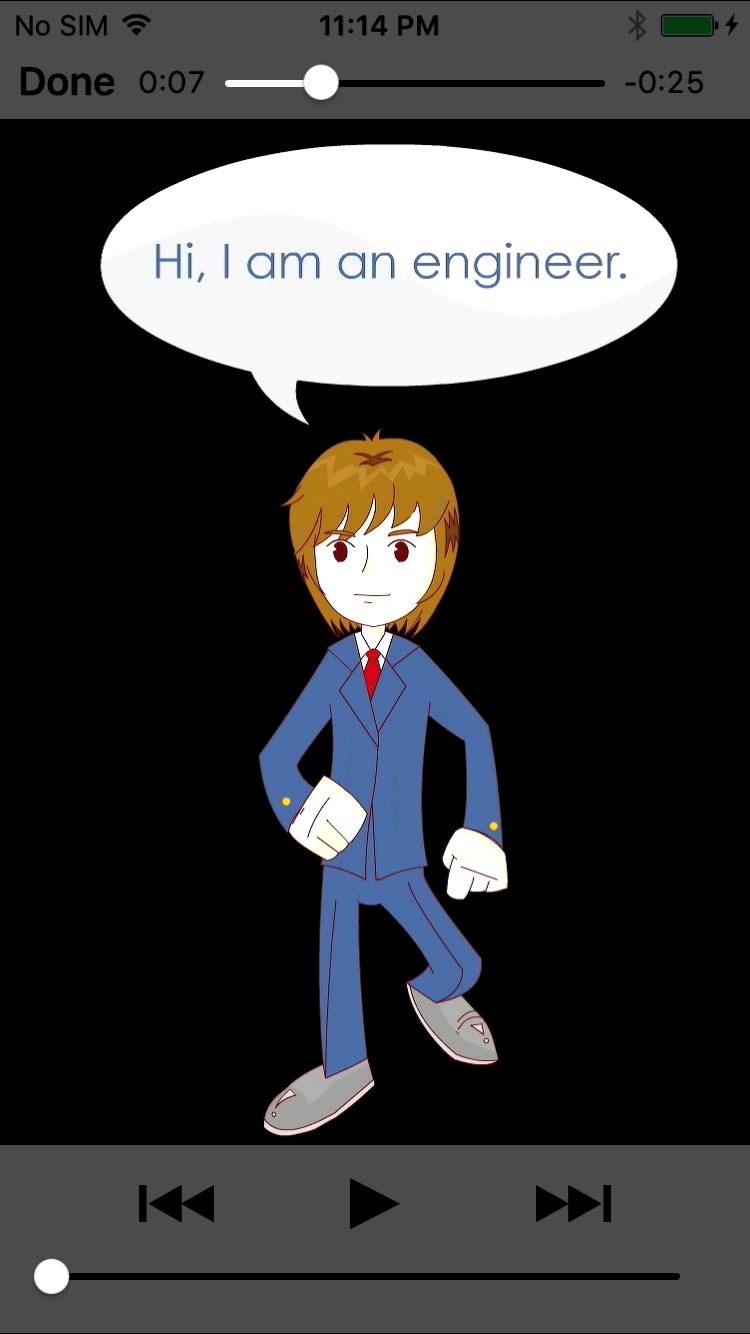
\includegraphics[width=\textwidth]{video2}
\caption{}
 \end{subfigure}\hspace{0.03\textwidth}
 \begin{subfigure}{0.25\textwidth}
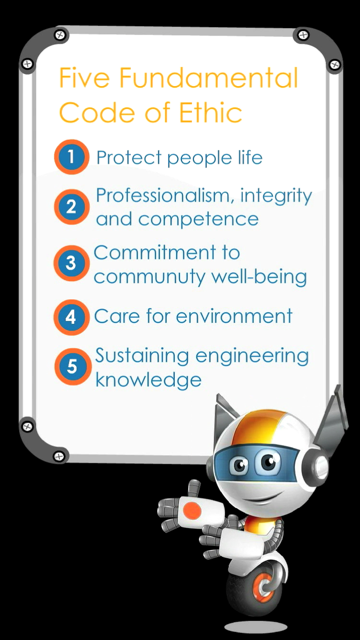
\includegraphics[width=\textwidth]{video3}
\caption{}
    \end{subfigure}\hspace{0.03\textwidth}
  \caption{Examples of animation video media that introduce learning topic}
\end{figure}

\newpage 
\subsubsection{5. Motivate learner}

We used rewarding (i.e., learners would received a grocery voucher if they perform all the learning support features provided in the application. Animation Video also was used in this matter, however, it was learners's desire if they would watch the video. 

\subsubsection{6. Allow learners to practice what they have learnt} 
Figure x presents the game based learning, we have score to give them feedback if they answered correctly. The chat icon also available on point for learners to contect their teachers if they wanted to discuss further issues

\begin{figure}[!hbt]\centering
    \begin{subfigure}{0.35\textwidth}
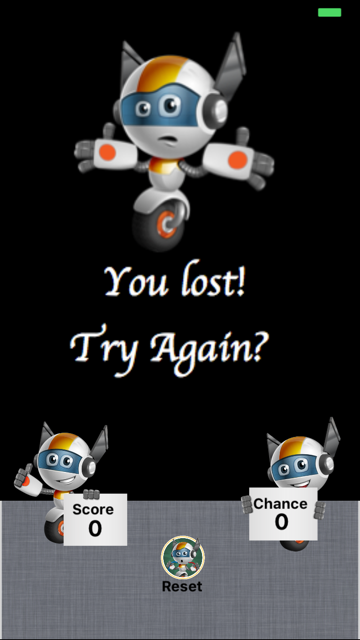
\includegraphics[width=\textwidth]{feed1}
\caption{}
    \end{subfigure}\hspace{0.06\textwidth}
 \begin{subfigure}{0.35\textwidth}

\includegraphics[width=\textwidth]{feed2}
\caption{}
 \end{subfigure}\hspace{0.5\textwidth}
  \caption{Feedback given in quize game}
\end{figure}

\newpage 
\subsubsection{7. Design for usability}
The text were presented with three different interface design techniques: pop-up, slide-menu, and dropped-down menu. 

\begin{figure}[!hbt]\centering
    \begin{subfigure}{0.3\textwidth}
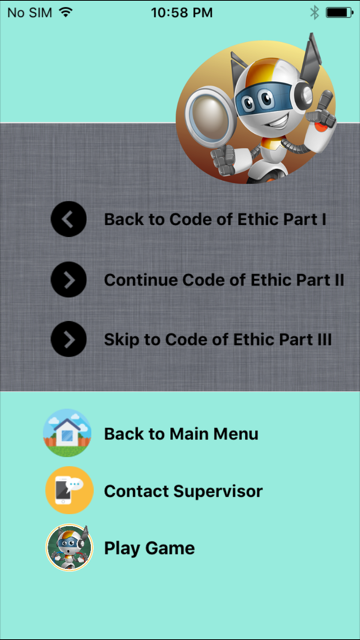
\includegraphics[width=\textwidth]{reverse}
\caption{Navigation}
    \end{subfigure}\hspace{0.02\textwidth}
 \begin{subfigure}{0.3\textwidth}
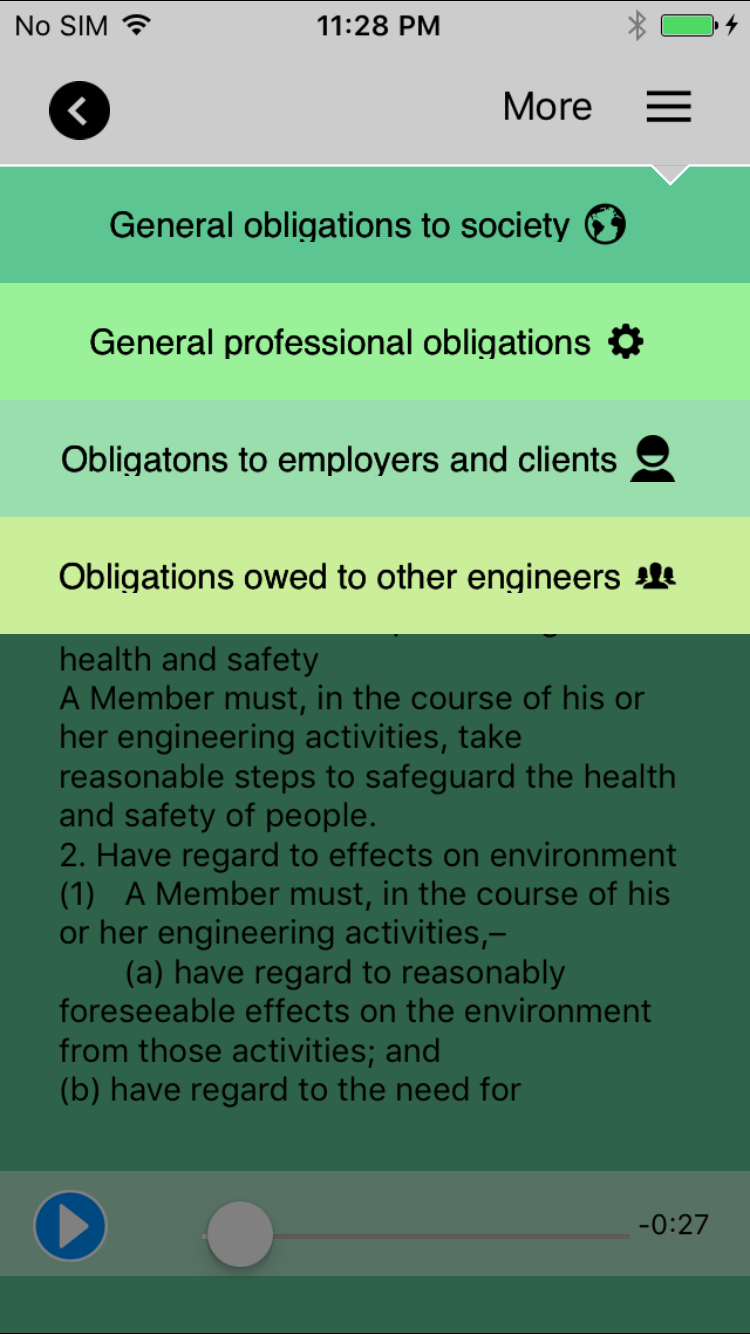
\includegraphics[width=\textwidth]{menu}
\caption{Drop-down menu}
 \end{subfigure}\hspace{0.02\textwidth}
 \begin{subfigure}{0.335\textwidth}
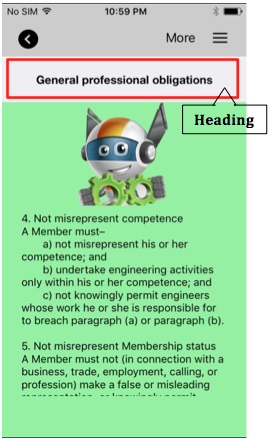
\includegraphics[width=\textwidth]{heading}
\caption{Heading}
 \end{subfigure}\hspace{0.06\textwidth}
  \caption{Usability design}
\end{figure}

\section{Summary} 
















